\documentclass[12pt,twoside,a4paper]{report}
\usepackage{amsmath}
\usepackage{amssymb}
\usepackage{mathabx}
\usepackage{graphicx}
\usepackage{fancyhdr}
\usepackage{enumerate}
\usepackage[vmargin=2.5cm, hmargin=2.5cm]{geometry}
\usepackage{hyperref}
\usepackage{fontspec}
\usepackage{unicode-math}
\usepackage{stackengine}
\usepackage{minitoc}
\usepackage{amsthm}
\usepackage{listings}
\usepackage{xcolor}
\usepackage{xeCJK}
\usepackage{dirtree}
\usepackage{float}
\usepackage{pdfpages}
\usepackage{atbegshi}


\setmainfont{Linux Libertine O}
\setsansfont{Linux Biolinum O}
\setCJKmainfont{Noto Serif CJK JP}

\graphicspath{{./fig/category_theory/}{./fig/agda/lagda/latex/}{./fig/implementation/}{./proposal/}{./code/}}

\setlength{\parindent}{0em}
\addtolength{\parskip}{1ex}

\usepackage[backend=biber,style=ieee]{biblatex}
\addbibresource{ref.bib}

\theoremstyle{definition}
\newtheorem{definition}{Definition}

\theoremstyle{definition}
\newtheorem{theorem}{Theorem}

\theoremstyle{definition}
\newtheorem{example}{Example}

\theoremstyle{definition}
\newtheorem{prf}{Proof}

\newcounter{motivation}
\renewcommand{\themotivation}{\Roman{motivation}}

\newcommand{\motivation}[1]{%
    \refstepcounter{motivation}%
    \vspace{1.5em}%
    \noindent\textbf{Motivation \themotivation.  #1}
    \par
    \expandafter\edef\csname savedmotivation\themotivation\endcsname{%
        \noexpand\noindent\noexpand\textbf{Motivation \themotivation. #1}\noexpand\par
    }%
}

\newcommand{\secref}[1]{\S\ref{#1}}
\newcommand{\chapref}[1]{\ref{#1}}

\definecolor{mediumblue}{HTML}{0000CD}
\definecolor{green}{HTML}{008B00}
\definecolor{orange}{HTML}{CD6600}
\definecolor{darkpink}{HTML}{EE1289}

\newcommand{\mb}[1]{\textcolor{mediumblue}{#1}}
\newcommand{\gn}[1]{\textcolor{green}{#1}}
\newcommand{\og}[1]{\textcolor{orange}{#1}}
\newcommand{\dpink}[1]{\textcolor{darkpink}{#1}}

\newcommand{\bN}{\mathbb{N}}

\newcommand{\yo}{\mathord{\text{\kern0.03em \scalebox{0.8}{よ}\kern0.03em}}}

\newcommand{\bracket}[1]{\left\{ #1 \right\}}
\newcommand{\ang}[1]{\left\langle #1 \right\rangle}

\newcommand{\frontmatter}{
  \pagenumbering{roman}
}

\newcommand{\mainmatter}{
  \cleardoublepage
  \pagenumbering{arabic}
  \setcounter{page}{1}
}

\begin{document}

\dominitoc

\begin{titlepage}
    \begin{flushright}
        \textbf{\Large Jack Gao}
    \end{flushright}
    
    \vspace{12em}

    \begin{center}
        \textbf{\huge Using functor categories to generate intermediate code with Agda}
        \vspace{3em}

        {\Large Computer Science Tripos - Part II Dissertation}
        \vspace{1em}

        {\Large Homerton College}
        \vspace{1em}

        {\large \today}
    \end{center}
\end{titlepage}

\begin{titlepage}
    \vspace*{5em}
    \textbf{\LARGE Declaration of Originality}
    \vspace{2em}

    I, the candidate for Part II of the Computer Science Tripos with Blind Grading Number 2330G, hereby declare that this report and the work described in it are my own work, unaided except as may be specified below, and that the report does not contain material that has already been used to any substantial extent for a comparable purpose. In preparation of this report, I adhered to the Department of Computer Science and Technology AI Policy. I am content for my report to be made available to the students and staff of the University.
    \vspace{1em}

    Date: \today
\end{titlepage}

\begin{titlepage}
    \vspace*{5em}
    \textbf{\LARGE Proforma}
    \vspace{2em}

    \begin{tabular}{ll}
        \textbf{Candidate Number:} & 2330G \\
        \textbf{Title of Project:} & Using functor categories to generate intermediate code with Agda \\
        \textbf{Examination} & Computer Science Tripos - Part II - 2025 \\
        \textbf{Word-Count:} & [wordcount] \\
        \textbf{Code line count:} & [linecount] \\
        \textbf{Project Originator:} & Yulong Huang \\
        \textbf{Project Supervisor:} & Yulong Huang and Yufeng Li \\
    \end{tabular}

    \vspace{2em}
    \textbf{\Large Original Aims of the Project}
    \vspace{1em}

    \vspace{2em}
    \textbf{\Large Work Completed}
    \vspace{1em}

    \vspace{2em}
    \textbf{\Large Special Difficulties}
    \vspace{1em}
\end{titlepage}

\frontmatter
\tableofcontents
\newpage

\mainmatter
\chapter{Introduction}
    \minitoc
    Programming languages act as a bridge between human thought and machine execution. They exist in two complementary realms: the human realm, where intent is expressed through abstractions like variables and functions, and the machine realm, where low-level instructions are executed on hardware. 

    Denotational semantics is related to the human realms. It provides a theoretical framework for defining the meaning of programming languages by interpreting them into mathematical objects. By formalising the denotational semantics of a programming language, we ensure that its abstraction align with human intuition. 

    Compilers are related to the machine realms. They are programs that translate high-level code into executable instructions, resolving abstractions into concrete operations like memory allocation and register management. Compilers are essential for turning human-written code into physical computation.

    This project explores how the two process can be deeply connected by demonstrating how denotational semantics can directly generate a compiler. Simple Typed Lambda Calculus (STLC) is a well-studied programming language that serves as a foundation for many modern languages. It has denotational semantics in cartesian closed categories, shown by Lambek~\cite{lambek}. As a ccc, presheaf categories over store locations can be used to model STLC with stores, as shown by by Reynolds~\cite{essence} and Oles~\cite{Oles_1}~\cite{Oles_2}. Instead, Reynolds~\cite{Reynolds} presented a denotational semantics of STLC with stores in the form of a presheaf category over compiler states. By interpresting the source language into the presheaf category over stack descriptors, where objects of the category represent instruction sequences parameterised by stack layouts, the semantic model directly yields a compiler. 
    
    I implement this compiler for STLC with stores in a dependently typed programming language, Agda~\cite{Agda}. The compiler is a functor (structure-preserving map) from the source language's semantic domain to the target language's instruction set. The implementation is verified with Agda's type system, which ensures that the generated code is well-typed and adheres to the semantics of both the source and target languages.

    This work both validates and refines Reynolds' theory, offering a concrete example of how category-theoretic semantics can generate intermediate code. The project also serves as a practical demonstration of the power of dependently typed programming languages can mechanise the link between theory and practice.

    \section{Motivation} \label{sec: motivation}
        This project is motivated and guided by the following:

        \motivation{Implementation of the compiler}
        Reynolds concluded that he did not have a proper dependently typed programming language in hand, so his compiler remained a partial function. I aim to provide a computer implementation of this theoretical framework in a dependently typed programming language.
        

        \motivation{Formal verification of the compiler}
        Reynolds' work presented detailed definitions of denotational semantics of STLC with stores, which are complicated and error-prone. The rise of verified compilers including CompCert~\cite{CompCert}, CakeML~\cite{CakeML} reflects a broader trend toward trustworthy systems, where correctness proofs replace testing for critical guarantees. I aim to provide a formalisation of the definition in a proof assistant to verify the correctness of the given denotational semantics.
        
        % \motivation{Trend of verified compilers}
        % The rise of verified compilers including CompCert~\cite{CompCert}, CakeML~\cite{CakeML} reflects a broader trend toward trustworthy systems, where correctness proofs replace testing for critical guarantees. Like Lean 4~\cite{Lean4}, we leverage dependent types to internalise the verification of correctness of terms.

    
    \section{Language choice: Agda's advantages}
        Agda~\cite{Agda} is a dependently typed programming language and proof assistant. Agda captures the source language's intrinsic sytax with indexed families, which contains only well-typed terms. Therefore, it focuses on the correct programs and rules out the ill-typed nonsensical inputs. 

        Dependently typed languages provide a natural framework for expressing functor categories is proven both theoretically and practically. There have been dependent-type-theoretic model of categories~\cite{Dybjer}, and it has been shown that functor categories arise naturally as dependent function types~\cite{Jacobs}. A formalisation of Category Theory, including cartesian closed categories, functors and presheaves has been developed in Agda by Hu and Caratte~\cite{Cat_Agda}. Other proof assistants, such as Isabelle/Hol, does not have a dependently typed language structure, and thus cannot express the functor categories as naturally as Agda. 

        Compared to other dependently typed languages, Agda is more balanced in terms of programming and proving. Its \og{\textsf{with}}-abstraction and \og{\textsf{rewrite}} construction allow for a more flexible and powerful way to define and manipulate terms. The \og{\textsf{with}}-abstraction allows us to inspect intermediate values in a term, which gives a refined view of a function's argument. The \og{\textsf{rewrite}} construction allows us to define new terms by expanding existing terms, which avoids rewriting proofs of similar structures.

        Agda also provides an interactive environment for writing and verifying programs, which will be further discussed in \secref{subsec: holes}.

    \section{Contributions}
        Addressed the three motivations presented in \secref{sec: motivation} and contributed to the following:
        \begin{quote}
            \savedmotivationI
            I implemented the compiler from the source language to the target language in Agda. 

            \savedmotivationII
            I formalised the terms in the source language and target language in Agda, and proved that the compiler is a functor from the source language to the target language. 

            % \savedmotivationIII
            % This implementation follows the trend of verified compilers, and provides a practical example of how to use functor categories to generate intermediate code.
        \end{quote}


\chapter{Preparation}
    \minitoc

    For implementing the compiler, I need to understand the theoretical background of presheaves and functor categories that are used as the denotational semantics of the source language, and I need to understand Agda's dependent types to correctly express the dependent function space of presheaf exponentials. This chapter begins with my starting point and an introduction to category theory, followed by a brief overview of the dependently typed programming language Agda, and requirements analysis of the compiler.

    \section{Starting Point}
    Prior to this project, I had no experience with Agda. Although I was aware of the open-source online tutorial \textit{Programming Language Foundations in Agda} (PLFA)~\cite{plfa}, my preparation was limited to setting up the Agda environment on my laptop by following the ``Front Matter'' section of the tutorial.

    I did not have any other experience with compiler beyond Part IB Compiler Construction Course. I had no prior exposure to category theory and type theory before the Part II lectures.


    \section{Category theory} \label{sec: cat}
        Category theory provides a high-level abstraction from which we can reason about the structure of mathematical objects and their relationships. It provides us a ``bird's eye view'' of the mathematics which enable us to spot patterns that are difficult to see in the details~\cite{basic_cat}. More specifically, it provides a ``purer'' view of functions that is not derived from sets~\cite{scott-lambda}. Compared to set theory which is ``element-oriented'', category theory is ``function-oriented'' and ``morphism-oriented''. We understand structures not via elements but by how they transform into each other. 

        Notation in category theory is similar to that in set theory and type theory. For example, $A, B, \dots$ are used to denote objects, sets, or types, and arrows are used to denote morphisms or functions (e.g.\ $A \to B$). There is a deeper connection between category theory and type theory, which will 
        be discussed in \secref{subsec: curry-howard-lambek}. 


        The following is a brief introduction to the basic concepts of category theory, which is based on the work of Leinster~\cite{basic_cat}, 
        Riehl~\cite{cat_context}, and the lecture notes of Part II Category Theory by Andrew Pitts and Marcelo Fiore~\cite{cat_lecture_notes}.

        \subsection{Category}
        \begin{definition}[Category]
            A \emph{category} $\mathcal{C}$ is specified by the following:
            \begin{itemize}
                \item 
                    a collection of objects $\textbf{obj}(\mathcal{C})$, whose elements are called $\mathcal{C}$-objects;
                \item 
                    for each $X, Y \in \textbf{obj}(\mathcal{C})$, a collection of morphisms $\mathcal{C}{(X,Y)}$, whose elements are called $\mathcal{C}$-morphisms from $X$ to $Y$ (e.g.\ $f : X \to Y$);
                \item 
                    for each $X \in \textbf{obj}(\mathcal{C})$, an element $\textbf{id}_X \in \mathcal{C}{(X,X)}$ called the identity morphism on $X$;
                \item 
                    for each $X, Y, Z \in \textbf{obj}(\mathcal{C})$, a function 
                    \[\begin{aligned}
                        \mathcal{C}{(X,Y)} \times \mathcal{C}{(Y,Z)} &\to \mathcal{C}{(X,Z)} \\
                        (f,g) &\mapsto g \circ f
                    \end{aligned}\]
                    called the composition of morphisms;
            \end{itemize}
            satisfying the following properties:
            \begin{itemize}
                \item 
                    \textbf{(Unit Laws)}
                    for all $X, Y \in \textbf{obj}(\mathcal{C})$ and $f \in \mathcal{C}{(X,Y)}$, we have:
                    \begin{equation} \label{law: unit}
                        \textbf{id}_Y \circ f = f = f \circ \textbf{id}_X
                    \end{equation}
                \item
                    \textbf{(Associativity Law)}
                    for all $X, Y, Z, W \in \textbf{obj}(\mathcal{C})$ and $f \in \mathcal{C}{(X,Y)}$, $g \in \mathcal{C}{(Y,Z)}$, $h \in \mathcal{C}{(Z,W)}$, we have:
                    \begin{equation} \label{law: associativity}
                        h \circ (g \circ f) = (h \circ g) \circ f
                    \end{equation}
            \end{itemize}
        \end{definition}

        \begin{example}[$\mathcal{Set}$]
            An example of category is the category of sets, denoted as $\mathcal{Set}$, specifed by:
            \begin{itemize}
                \item 
                    the objects of $\mathcal{Set}$ are a fixed universe of sets;
                \item
                    for each $X, Y \in \textbf{obj}(\mathcal{Set})$, the morphisms from $X \to Y$ in $\mathcal{Set}$ are the functions $X \to Y$;
                \item
                    the identity morphism on $X$ in $\mathcal{Set}$ is the identity function on $X$;
                \item
                    the composition of morphisms in $\mathcal{Set}$ is defined as the composition of functions.
            \end{itemize}
            Associativity law and unit laws are satisfied in $\mathcal{Set}$, since the composition of functions is associative and the identity function compose with any function is the function itself.
        \end{example}

        \begin{example}[$\mathcal{Poset}$]
            Another example of category is the category of posets, denoted as $\mathcal{Poset}$, specified by:
            \begin{itemize}
                \item 
                    the objects of $\mathcal{Poset}$ are a fixed universe of posets, which is a set $P$ with a binary relation $\subseteq$ that is 
                    \begin{itemize}
                        \item reflexive: $\forall x \in P, x \subseteq x$;
                        \item transitive: $\forall x, y, z \in P, x \subseteq y \land y \subseteq z \implies x \subseteq z$;
                        \item antisymmetric: $\forall x, y \in P, x \subseteq y \land y \subseteq x \implies x = y$.
                    \end{itemize}
                \item
                    for each $X, Y \in \textbf{obj}(\mathcal{Poset})$, the morphisms from $X$ to $Y$ in $\mathcal{Poset}$ are the monotone (order-preserving) functions from $X$ to $Y$;
                \item
                    the identity morphism on $X$ in $\mathcal{Poset}$ is the identity function on $X$;
                \item
                    the composition of morphisms in $\mathcal{Poset}$ is defined as the composition of functions.
            \end{itemize}
            Associativity law and unit laws are satisfied in $\mathcal{Poset}$, since the set of monotone functions contains identity functions and is closed under composition.

            $\mathcal{Poset}$ is used later for stack descriptors in the denotational semantics of the source language.
        \end{example}

            \subsubsection{Opposite category}
            The idea of opposite category is that if we have a category $\mathcal{C}$, we can reverse the direction of all morphisms in $\mathcal{C}$ to obtain a new category $\mathcal{C}^{\textbf{op}}$.

            \begin{definition}[Opposite category]
                Given a category $\mathcal{C}$, its \emph{opposite category} $\mathcal{C}^{\textbf{op}}$ is specified by:
                \begin{itemize}
                    \item 
                        the objects of $\mathcal{C}^{\textbf{op}}$ are the same as those of $\mathcal{C}$;
                    \item 
                        for each $X, Y \in \textbf{obj}(\mathcal{C})$, the morphisms from $X$ to $Y$ in $\mathcal{C}^{\textbf{op}}$ are the morphisms from $Y$ to $X$ in $\mathcal{C}$;
                    \item 
                        the identity morphism on $X$ in $\mathcal{C}^{\textbf{op}}$ is the identity morphism on $X$ in $\mathcal{C}$;
                    \item 
                        the composition of morphisms in $\mathcal{C}^{\textbf{op}}$ is defined as the composition of morphisms in $\mathcal{C}$.
                \end{itemize}
            \end{definition}

                % \paragraph{The principle of duality}
                % Whenever one defines a concept or proves a theorem in category theory $\mathcal{C}$, one can obtain another concept or theorem in the opposite category $\mathcal{C}^{\textbf{op}}$, called the \emph{dual} of the original concept or theorem, by reversing all arrows in the original concept or theorem.

            The notation of commutative diagram is widely used in category theory as a convenient visual representation of the relationships between objects and morphisms in a category.
            \subsubsection{Commutative diagrams}
            A \emph{diagram} in a category $\mathcal{C}$ is a directed graph whose vertices are $\mathcal{C}$-objects and whose edges are $\mathcal{C}$-morphisms.

            A diagram is \emph{commutative} (or \emph{commutes}) if any two finite paths in the graph between any two vertices $X$ and $Y$ in the diagram determine the equal morphism $f \in \mathcal{C}{(X,Y)}$ under the composition of morphisms.

            \begin{figure}[H]
                \centering
                \begin{minipage}{0.3\textwidth}
                    \centering
                    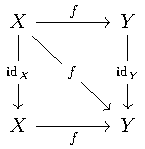
\includegraphics[width=0.8\textwidth]{unit_laws.pdf}
                    \caption{Commutative diagram for Unit Laws}
                    \label{fig: unit_laws}
                \end{minipage} \hspace{0.2\textwidth}
                \begin{minipage}{0.3\textwidth}
                    \centering
                    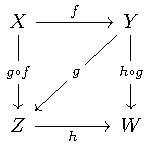
\includegraphics[width=0.8\textwidth]{associativity_law.pdf}
                    \caption{Commutative diagram for Associativity Law}
                    \label{fig: associativity_law}
                \end{minipage}
            \end{figure}

            As examples of commutative diagrams, Figure \ref{fig: associativity_law} and Figure \ref{fig: unit_laws} are commutative diagrams for the unit laws and associativity law respectively. 

        
        \subsection{Isomorphism}
        \begin{definition}[Isomorphism]
            Given a category $\mathcal{C}$, a $C$-morphism $f : X \to Y$ is called an \emph{isomorphism} if there exists a $C$-morphism $g : Y \to X$ such that the following diagram commutes:
            \begin{equation}
                \vcenter{\hbox{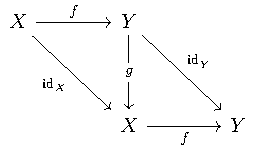
\includegraphics[width=0.3\textwidth]{isomorphism.pdf}}}
                \label{cd: isomorphism}
            \end{equation}
            In other words, $f$ is an isomorphism if there exists a morphism $g$ such that $g \circ f = \textbf{id}_X$ and $f \circ g = \textbf{id}_Y$.

            The morphism $g$ is uniquely determined by $f$ and is called the \emph{inverse} of $f$, denoted as $f^{-1}$.

            Given two objects $X$ and $Y$ in a category $\mathcal{C}$, if there exists an isomorphism from $X$ to $Y$, we say that $X$ and $Y$ are \emph{isomorphic} in $\mathcal{C}$ and write $X \cong Y$.

        \end{definition}

        \subsection{Cartesian closed category}
            \subsubsection{Terminal object}
            \begin{definition}[Terminal object]
                Given a category $\mathcal{C}$, an object $T \in \textbf{obj}(\mathcal{C})$ is called a \emph{terminal object} if for all $X \in \textbf{obj}(\mathcal{C})$, there exists a unique \textbf{C}-morphism $f : X \to T$.
            \end{definition}
            Terminal objects are unique up to isomorphism. In other words, we have
            \begin{itemize}
                \item 
                    if $T$ and $T'$ are both terminal objects in $\mathcal{C}$, then there exists a unique isomorphism $f : T \to T'$.
                \item
                    if $T$ is a terminal object in $\mathcal{C}$ and $T \cong T'$, then $T'$ is also a terminal object in $\mathcal{C}$.
            \end{itemize}
            \begin{example}[Terminal object in $\mathcal{Set}$]
                $\mathcal{Set}$ has a terminal object $\{\ast\}$, which is an arbitrary singleton set containing a single element $\ast$.

                For any set $X$, there exists a unique function $f : X \to \{\ast\}$ that maps every element of $X$ to the single element $\ast$ in $\{\ast\}$.
                
                There is a unique isomorphism $f : \{\ast\} \to \{\cdot\}$ for any two singleton sets $\{\ast\}$ and $\{\cdot\}$, which is $f(\ast) = \cdot$.
            \end{example}

            
            \subsubsection{Binary product}
            \begin{definition}[Binary product]
                Given a category $\mathcal{C}$, the \emph{binary product} of two objects $X$ and $Y$ in $\mathcal{C}$ is specified by
                \begin{itemize}
                    \item a $\mathcal{C}$-object $X \times Y$;
                    \item two $\mathcal{C}$-morphisms $\pi_1 : X \times Y \to X$ and $\pi_2 : X \times Y \to Y$ called the \emph{projections} of $X \times Y$;
                \end{itemize}
                such that for all $Z \in \textbf{obj}(\mathcal{C})$ and morphisms $f : Z \to X$ and $g : Z \to Y$, there exists a unique morphism $u : Z \to X \times Y$ such that the following diagram commutes in $\mathcal{C}$:
                \begin{equation}
                    \vcenter{\hbox{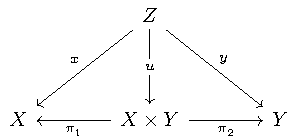
\includegraphics[width=0.4\textwidth]{binary_product.pdf}}}
                    \label{cd: binary_product}
                \end{equation}
                The unique morphism $u$ is written as 
                \[ \bracket{ f, g } : Z \to X \times Y \]
                where $f = \pi_1 \circ u$ and $g = \pi_2 \circ u$.
            \end{definition}
            It can be shown that the binary product is unique up to (unique) isomorphism.

            \begin{example}[Binary product in $\mathcal{Set}$]
                The binary product of two sets $X$ and $Y$ in $\mathcal{Set}$ is the Cartesian product $X \times Y = \{(x,y) \mid x \in X \land y \in Y\}$, where $(x,y)$ are ordered pairs.

                We have the following projections:
                \begin{itemize}
                    \item 
                        $\pi_1 : X \times Y \to X$ is defined as $\pi_1(x,y) = x$ for all $(x,y) \in X \times Y$;
                    \item
                        $\pi_2 : X \times Y \to Y$ is defined as $\pi_2(x,y) = y$ for all $(x,y) \in X \times Y$.
                \end{itemize}

            
                For any set $Z$, for any functions $f : Z \to X$ and $g : Z \to Y$, the unique morphism $u : Z \to X \times Y$ is defined as:
                \[u(z) = (f(z), g(z)) \text{ for all $z \in Z$.}\]
            \end{example}



            \subsubsection{Exponential}
            \begin{definition}[Exponential]
                Given a category $\mathcal{C}$ with binary products, the \emph{exponential} of two objects $X$ and $Y$ in $\mathcal{C}$ is specified by
                \begin{itemize}
                    \item a $\mathcal{C}$-object $X \Rightarrow Y$;
                    \item a $\mathcal{C}$-morphism $\textbf{app} : (X \Rightarrow Y) \times X \to Y$ called the \emph{application} of $X \Rightarrow Y$;
                \end{itemize}
                such that for all $Z \in \textbf{obj}(\mathcal{C})$ and morphisms $f : Z \times X \to Y$, there exists a unique morphism $u : Z \to X \Rightarrow Y$ such that the following diagram commutes in $\mathcal{C}$:
                \begin{equation}
                    \vcenter{\hbox{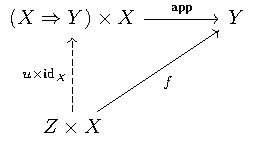
\includegraphics[width=0.4\textwidth]{exponential.pdf}}}
                    \label{cd: exponential}
                \end{equation}
                We write $\textbf{cur} f$ for the unique morphism $u$ such that $f = \textbf{app} \circ (\textbf{cur} f \times \textbf{id}_X)$, 
                where $\textbf{cur} f$ is called the \emph{currying} of $f$.
            \end{definition}
            It can be shown that the exponential is unique up to (unique) isomorphism.

            \begin{example}[Exponential in $\mathcal{Set}$]
                The exponential of two sets $X$ and $Y$ in $\mathcal{Set}$ is the set of all functions from $X$ to $Y$.

                Function application gives the morphism $\textbf{app} : (X \Rightarrow Y) \times X \to Y$ as $\textbf{app}(f,x) = f(x)$ for all $f \in X \Rightarrow Y$ and $x \in X$.

                The currying operation transform a function $f : Z \times X \to Y$ into a function $\textbf{cur} f : Z \to (X \Rightarrow Y)$, which is defined as $\textbf{cur} f(z) = \lambda x.f(z,x)$ for all $z \in Z$ and $x \in X$.

                
            \end{example}

        \begin{definition}[Cartesian closed category]
            A category $\mathcal{C}$ is called a \emph{Cartesian closed category} (ccc) if it has a terminal object, binary products and exponentials of any two objects.
        \end{definition}

        
        \subsection{Functor}
        \begin{definition}[Functor]
            Given two categories $\mathcal{C}$ and $\mathcal{D}$, a \emph{functor} $F: \mathcal{C} \to \mathcal{D}$ is specified by:
            \begin{itemize}
                \item 
                    a function 
                    \[\begin{aligned}
                        \textbf{obj}(\mathcal{C}) &\to \textbf{obj}(\mathcal{D}) \\
                        X &\mapsto F(X)
                    \end{aligned}\]

                \item 
                    for each $X, Y \in \textbf{obj}(\mathcal{C})$, a function 
                    \[\begin{aligned}
                        \mathcal{C}{(X,Y)} &\to \mathcal{D}{(F(X),F(Y))} \\
                        f &\mapsto F(f)
                    \end{aligned}\]
            \end{itemize}
            satisfying the following properties:
            \begin{itemize}
                \item 
                    for all $X, Y \in \textbf{obj}(\mathcal{C})$ and $f \in \mathcal{C}{(X,Y)}$, we have: $ F(\textbf{id}_X) = \textbf{id}_{F(X)}$
                \item
                    for all $X, Y, Z \in \textbf{obj}(\mathcal{C})$ and $f \in \mathcal{C}{(X,Y)}$, $g \in \mathcal{C}{(Y,Z)}$, we have: $F(g \circ f) = F(g) \circ F(f)$
            \end{itemize}
        \end{definition}

        
        \subsection{Natural transformation}
        \begin{definition}[Natural transformation]

            Given two categories $\mathcal{C}$ and $\mathcal{D}$, and two functors $F,G: \mathcal{C} \to \mathcal{D}$, a \emph{natural transformation} $\theta : F \to G$ is a family of morphisms $\theta_X \in \mathcal{D}{(F(X),G(X))}$ for each $X \in \textbf{obj}(\mathcal{C})$ such that for all $X, Y \in \textbf{obj}(\mathcal{C})$ and $f \in \mathcal{C}{(X,Y)}$, the following diagram 
            \begin{equation}
                \vcenter{\hbox{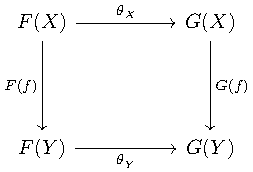
\includegraphics[width=0.3\textwidth]{natural_transformation.pdf}}}
                \label{cd: natural_transformation}
            \end{equation}
            
            commutes in $\mathcal{D}$, i.e. $G(f) \circ \theta_X = \theta_Y \circ F(f)$

        \end{definition}

        
        \subsection{Functor category}
        \begin{definition}[Functor category]
            Given two categories $\mathcal{C}$ and $\mathcal{D}$, the \emph{functor category} $\mathcal{D}^{\mathcal{C}}$ is the category satisfying the following:
            \begin{itemize}
                \item 
                    the objects of $\mathcal{D}^{\mathcal{C}}$ are all functors $\mathcal{C} \to \mathcal{D}$;
                \item 
                    given two functors $F,G: \mathcal{C} \to \mathcal{D}$, the morphisms from $F$ to $G$ in $\mathcal{D}^{\mathcal{C}}$ are all natural transformations $\theta : F \to G$;
                \item
                    composition and identity morphisms in $\mathcal{D}^{\mathcal{C}}$ are defined as follows:
                    \begin{itemize}
                        \item 
                            the identity morphism $\textbf{id}_F$ on $F$ is defined as $\theta_X = \textbf{id}_{F(X)}$ for all $X \in \textbf{obj}(\mathcal{C})$;
                        \item
                            the composition of two natural transformations $\theta : F \to G$ and $\phi : G \to H$ is defined as $(\phi \circ \theta)_X = \phi_X \circ \theta_X$ for all $X \in \textbf{obj}(\mathcal{C})$.
                    \end{itemize}
            \end{itemize}
        \end{definition}

        \subsection{Presheaf category}
        \begin{definition}[Presheaf]
            Given a category $\mathcal{C}$, a \emph{presheaf} on $\mathcal{C}$ is a functor $F: \mathcal{C}^{\textbf{op}} \to \textbf{Set}$.
            A presheaf is a contravariant functor, which means that it reverses the direction of morphisms.
            In other words, a presheaf is a functor that takes objects in $\mathcal{C}$ and assigns them sets, and takes morphisms in $\mathcal{C}$ and assigns them functions between the corresponding sets.
            The presheaf $F$ is defined as follows:
            \begin{itemize}
                \item 
                    for each $X \in \textbf{obj}(\mathcal{C})$, $F(X)$ is a set;
                \item
                    for each $X, Y \in \textbf{obj}(\mathcal{C})$ and $f \in \mathcal{C}{(X,Y)}$, $F(f)$ is a function $F(Y) \to F(X)$.
            \end{itemize}
        \end{definition}

        \begin{definition}[Presheaf category]
            Given a category $\mathcal{C}$, the \emph{presheaf category} $\hat{\mathcal{C}}$ is the is the functor category $\mathcal{Set}^{\mathcal{C}^{\textbf{op}}}$, which explicitly contains the following:
            \begin{itemize}
                \item 
                    the objects of $\hat{\mathcal{C}}$ are all presheaves on $\mathcal{C}$;
                \item
                    given two presheaves $F,G: \mathcal{C}^{\textbf{op}} \to \mathcal{Set}$, the morphisms from $F$ to $G$ in $\hat{\mathcal{C}}$ are all natural transformations $\theta : F \to G$.
            \end{itemize}
        \end{definition}



        \subsection{Yoneda lemma}
        \begin{definition}[Yoneda functor]
            Given a category $\mathcal{C}$, the \emph{Yoneda functor} $\yo: \mathcal{C} \to \hat{\mathcal{C}}$ is defined as follows:
            \begin{itemize}
                \item 
                    for each $X \in \textbf{obj}(\mathcal{C})$, $\yo(X)$ is the functor $\mathcal{C}^{\textbf{op}} \to \mathcal{Set}$ defined as:
                    \begin{equation} \label{eq: yoneda_element}
                        \yo(X)(Y) = \mathcal{C}{(Y,X)}
                    \end{equation}
                    for all $Y \in \textbf{obj}(\mathcal{C})$;
                \item
                    for each $X, Y \in \textbf{obj}(\mathcal{C})$ and $f \in \mathcal{C}{(X,Y)}$, $\yo(f)$ is the morphism $\yo(X) \to \yo(Y)$ defined a natural transformation whose component at any given $Z \in \mathcal{C}^{\textbf{op}}$ is given by:
                    \begin{equation} \label{eq: yoneda_morphism}
                        \begin{aligned}
                            (\yo(f))_Z : \mathcal{C}{(Z,Y)} &\to \mathcal{C}{(Z,X)} \\
                            g &\mapsto g \circ f
                        \end{aligned}
                    \end{equation}
                    for all $Z \in \textbf{obj}(\mathcal{C})$.
                \end{itemize}

        \end{definition}

        \begin{theorem}[Yoneda lemma]
            Given a category $\mathcal{C}$, the \emph{Yoneda lemma} states that for each object $X \in \textbf{obj}(\mathcal{C})$ and any functor $F: \mathcal{C} \to \textbf{Set}$, there is a natural isomorphism:
            \begin{equation} \label{eq: yoneda_lemma}
                {\hat{\mathcal{C}}}(\yo(X), F) \cong F(X)
            \end{equation}
        \end{theorem}



        \subsection{Cartesian closed structure in presheaf categories}
        \begin{prf}[Cartesian closed structure in presheaf categories]
            Given a small category $\mathcal{C}$, the presheaf category $\hat{\mathcal{C}}$ is a Cartesian closed category.
            \begin{itemize}
                \item 
                    The terminal object in $\hat{\mathcal{C}}$ is the constant functor $\mathbf{1} : \mathcal{C}^{\textbf{op}} \to \mathcal{Set}$, given by 
                    \begin{equation}
                        \begin{cases}
                            \mathbf{1}(X) = \{\ast\} & \text{for all } X \in \textbf{obj}(\mathcal{C}) \\
                            \mathbf{1}(f) = \textbf{id}_{\{\ast\}} & \text{for all } f \in \mathcal{C}{(X,Y)}
                        \end{cases}
                    \end{equation}

                \item
                    The binary product in $\hat{\mathcal{C}}$ is given by the product of functors, which is defined as follows:
                    \begin{equation}
                        \begin{aligned}
                            (F \times G)(X) &= F(X) \times G(X) \\
                            (F \times G)(f) &= F(f) \times G(f)
                        \end{aligned}
                    \end{equation}

                \item
                    The exponential in $\hat{\mathcal{C}}$ is derived from the Yoneda lemma,
                    \begin{equation}
                        \begin{aligned}
                            G^{F}(X) &= \hat{\mathcal{C}}(\yo(X) \times F, G) \\
                            G^{F}(f)(\theta) &= \theta \circ (\yo(f) \times \textbf{id}_F) \quad \text{for all } \theta \in \hat{\mathcal{C}}(\yo(Y) \times F, G)
                        \end{aligned}
                    \end{equation}
            \end{itemize}
        \end{prf}
        


    \section{Agda}
        \subsection{Basic datatypes and pattern matching}
        We will go through a simple example in PLFA~\cite{plfa} to illustrate the basic datatypes and pattern matching in Agda.

        \[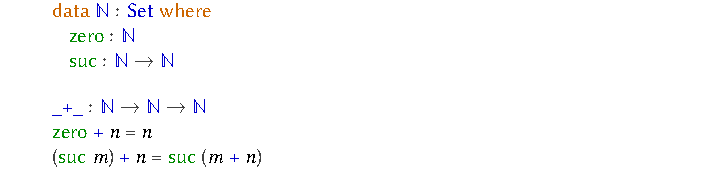
\includegraphics[scale=1.2]{natural_plus.pdf}\]

        Here we define a datatype $\mb{\bN}$ for natural numebers. $\mb{\bN}$ itself has a type $\mb{\mathsf{Set}}$, which is the type of all small types. The natural number is defined as a recursive datatype with two constructors: $\gn{\mathsf{zero}}$ and $\gn{\mathsf{suc}}$, where 
        $\gn{\mathsf{zero}}$ is the base case and $\gn{\mathsf{suc}}$ is the inductive case. The $\gn{\mathsf{zero}}$ constructor has type $\mb{\bN}$, and the $\gn{\mathsf{suc}}$ constructor has type $\mb{\bN \to \bN}$.

        In order to define the plus function $\mb{\_+\_}$, we use pattern matching to match the input argument with the constructors of the datatype. The first case is the base case, where we match the input argument with $\gn{\mathsf{zero}}$. In this case, we return the second argument. The second case is the inductive case, where we match the input argument with $\gn{\mathsf{suc}}$. In this case, we return $\gn{\mathsf{suc}}$ applied to the result of adding one to the second argument.

        \subsection{Dependent Types}
        A dependent type is a type that depends on a value. In terms of type judgement, simple types are in form of
        \[ x_1 : T_1, x_2 : T_2, \dots, x_n : T_n \vdash t(x_1, \dots, x_n) : T \]
        In contrast, dependent types are in form of
        \[ x_1 : T_1, x_2 : T_2, \dots, x_n : T_n \vdash t(x_1, \dots, x_n) : T(x_1, \dots, x_n) \]
        or more generally
        \[ x_1 : T_1, x_2 : T_2(x_1), \dots, x_n : T_n(x_1, \dots, x_{n-1}) \vdash t(x_1, \dots, x_n) : T(x_1, \dots, x_n) \]

        A classical example of dependent types in Agda is the type of vectors, which are lists with a length. 

        \[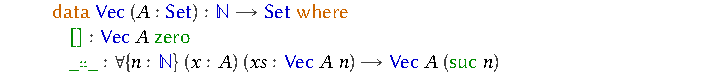
\includegraphics[scale=1.2]{vector.pdf}\]

        Here we define a datatype $\mb{\mathsf{Vec}}$ for vectors. The type of vectors is dependent on the length of the vector. With dependent types, we can encode properties directly into types and ensure that they are satisfied at compile time.

        \subsection{Curry-Howard-Lambek correspondence} \label{subsec: curry-howard-lambek}
        Curry-Howard correspondence~\cite{curry-howard} establishes an isomorphism between logic and type theory, where propositions correspond to types and proofs correspond to terms. This correspondence forms the foundation of functional programming languages that can be used to implement proofs. Building upon this, Joachim Lambek showed that cartesian closed categories provide a natural semantic setting for the simply typed lambda calculus (STLC)~\cite{lambek}. The Curry-Howard-Lambek correspondence can be summarised as follows:
        \begin{table}[H]
            \centering
            \begin{tabular}{|c|c|c|}
                \hline
                \textbf{Logic} & \textbf{Type theory} & \textbf{Category theory} \\
                \hline
                Proposition & Type & Object \\
                Proof & Term & Morphism \\
                Falsity & Empty type & Initial object \\
                Truth & Unit type & Terminal object \\
                Implication & Function type & Exponential \\
                Conjunction & Product type & Product \\
                Disjunction & Sum type & Coproduct \\
                % Universal quantification & Dependent product type &  \\
                % Existential quantification & Dependent sum type &  \\
                \hline
            \end{tabular}
            \caption{Curry-Howard-Lambek correspondence}
            \label{tab: curry-howard-lambek}
        \end{table}

        \subsection{Equality, congruence and substitution}\label{subsec: equality}
        Equality here refers to the propositional equality. In Agda it is defined as
        \[
\includegraphics[scale=1.2]{equality.pdf}\]
        With equality as a type, whenever we want to prove that two terms are equal, we need to provide a witness of the equality. For example if we want to prove $x \equiv y$, we write out a term of type $\mb{\mathsf{x = y}}$, and then give its definition, which constructs a proof of the equality. A simple proof that directly uses the definition of equality is as follows:
        \[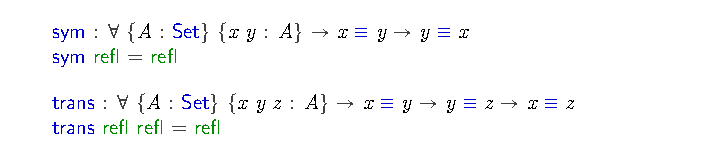
\includegraphics[scale=1.2]{sym_trans.pdf}\]
        Here we are able to prove the symmetry and transitivity of equality by using the definition of equality. Those two properties are very useful for later proofs. 

        We can also have more complex proof with congruence and substitution, which can also be directly derived from the definition of equality as follows:
        \[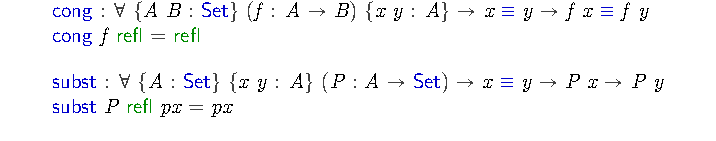
\includegraphics[scale=1.2]{cong_subst.pdf}\]
        Congruence is a property of equality that states that if two terms are equal, then they can be substituted for each other in any context. Substitution is a property where we can get a new proof by replacing a term in a proof with another term that is equal to it. 

        Here is a simple example of how congruence can be used in a proof:
        \[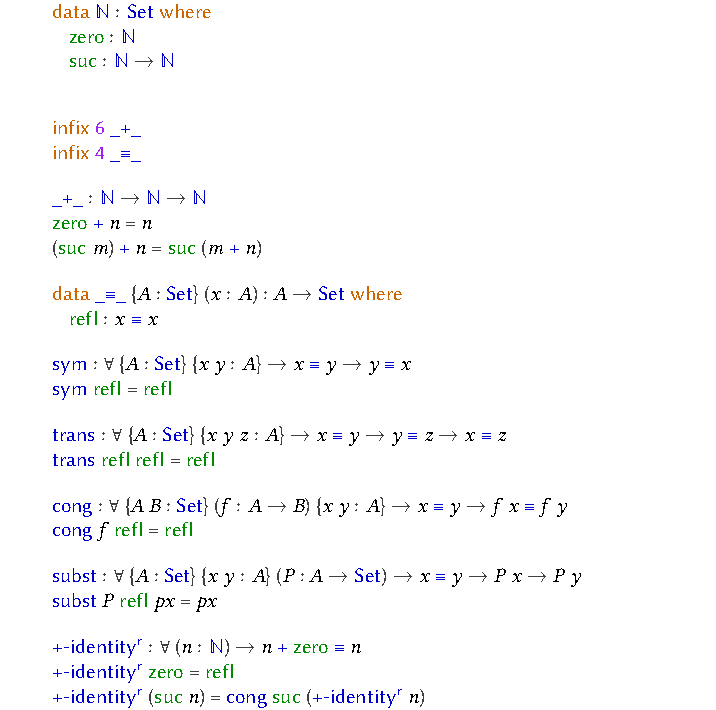
\includegraphics[scale=1.2]{cong_example.pdf}\]

        In this example, we want to prove that $\gn{\mathsf{zero}}$ is the right identity of the plus function. We do an inductive proof by pattern matching on the first argument of the plus function. 
        
        In the base case, we have $\gn{\mathsf{zero}} \mb{{}+{}} \gn{\mathsf{zero}} \equiv \gn{\mathsf{zero}}$, which is trivially true by the definition of the plus function (zero is defined to be the left identity of the plus function). 
        
        In the inductive case, we need to show $\gn{\mathsf{suc}}\ n \mb{{}+{}} \gn{\mathsf{zero}} \equiv \gn{\mathsf{suc}}\ n$. We can use the definition of the plus function to rewrite the left-hand side as $\gn{\mathsf{suc}}\ (n \mb{{}+{}} \gn{\mathsf{zero}})$. By the inductive hypothesis, we know that $n \mb{{}+{}} \gn{\mathsf{zero}} \equiv n$, so we can substitute $n$ for $n \mb{{}+{}} \gn{\mathsf{zero}}$ in the right-hand side by congruence, and we are done.

        % \subsection{With and Rewrite}

        \subsection{Standard library}
        The Agda standard library~\cite{agda_std} is a collection of modules that provide a wide range of useful functions and types. It includes modules for basic data types, such as natural numbers, lists, and vectors. In my implementation, however, I defined most of the basic data types and functions from scratch for the following two reasons:
        \begin{itemize}
            \item
                I wanted to have a better understanding of the basic data types and functions, so I decided to implement them from scratch.
            \item
                I need a particular representation of minus operation that ensures the input is always valid. This is further explained in [to add]
        \end{itemize}

        \subsubsection{Builtin pragma} \label{subsubsec: builtin_pragma}
        With standard library, we can use actual numbers $1, 2, 3, \dots$ instead of calling the constructor $\gn{\mathsf{suc}}$ multiple times. This is a convenient feature for testing. Agda provides a way to link self-defined functions to the standard library with a \og{\textsf{BUILTIN}} pragma. This allows me to use a convenient syntax for numbers, while still using the self-defined functions in the implementation.
        \[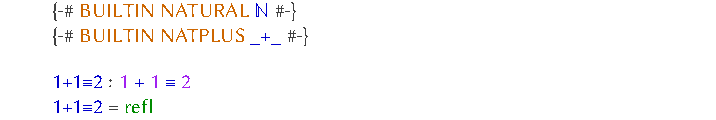
\includegraphics[scale=1.2]{natural_pragma.pdf}\]
        Note that in agda we can use unicode characters for terms, which makes the code more readable. For example, here we simply name the term \mb{1+1$\equiv$2}.

        
        \subsection{Interactive programming with holes} \label{subsec: holes}
        A feature of Agda is that it allows us to write programs with holes interatively. A hole is a placeholder for a term that we have not yet defined. By leaving holes in place of undefined terms, we can write programs that are incomplete but still type-check, and Agda's type checker will guide completion of the program: the context window displays inferred types of the holes, available variables and candidate terms with their types. Holes also supports case split and refinement, which means we can fill in a hole partially and split it into smaller holes. 

        In my implementation, I used holes to write the terms in the compiler. The complex terms are incrementally filled and verified by interatively refining partial implementations, reducing post-hoc debugging and ensuring robustness.


    \section{Requirement Analysis}
    To complete a compiler in Agda we need to implement the following components:
    \begin{itemize}
        \item 
            A file source.agda that record the syntax of the source language.

        \item
            A file target.agda that record the syntax of the target language.

        \item
            A file compiler.agda that uses source.agda and target.agda as modules, and write functions whose input is a term in the source language and output is a term in the target language.
    \end{itemize}
    The success criteria of the project is that the compiler can compile a term in the source language to a term in the target language, and the output term is well-typed in the target language.

\chapter{Implementation} \label{chap: implementation}
    \minitoc
    This chapter details the implementation of the compiler in Agda. Starting with a brief overview of the tools used, it then describes the directory structure and file dependencies. Then it discusses the specification of the source language, and the target language, which lead us to the problem of implementing a rigorous natural number subtraction and two different approaches. We will further see the difference between the two approaches and how they affect the implementation of the customised library and the implementation of the compiler. 
    

    \section{Tools used}
    The project is implemented in Agda 2.7.0.1, which is the latest stable version at the time of writing.

    Completing the project is an iterative process. I used Git~\cite{git} for version control, and work had been synchronised with a GitHub~\cite{github} repository for backup.

    For the development environment, I tried both Emacs~\cite{emacs} and Visual Studio Code~\cite{vscode} with an agda-mode extension~\cite{agda_mode} on Windows Subsystem for Linux with Ubuntu~\cite{wsl_ubuntu} 22.04 LTS. I am more familiar with the snippet and syntax highlighting features of Visual Studio Code, so I used it for most of the development. 

    Code from the PLFA tutorial and Agda standard library~\cite{agda_std} were used as references for implementation of the source language and the customised library. Apart from that, the code is written from scratch.

    \section{Repository Overview}
        \subsection{Directory structure}
        The repository contains two independent implementations of the compiler, organised as follows:
        \dirtree{%
            .1 ..
            .2 fin.
            .3 lib.agda.
            .3 source.agda.
            .3 target.agda.
            .3 compiler.agda.
            .2 proof.
            .3 lib.agda.
            .3 source.agda.
            .3 target.agda.
            .3 compiler.agda.
        }

        \subsection{File dependencies and descriptions}
        The dependency graph for each implementation is identical as follows:
        \begin{figure}[H]
            \centering
            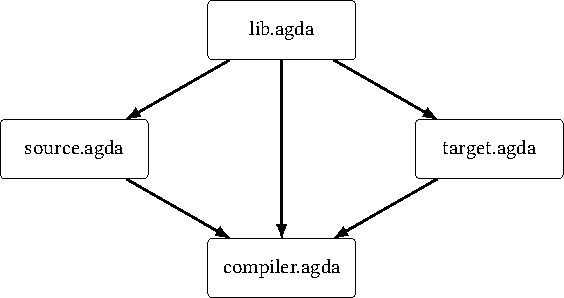
\includegraphics[width=0.6\textwidth]{dependencies.pdf}
            \caption{Dependency graph for the compiler}
            \label{fig: dependencies}
        \end{figure}

        \begin{table}[H]
            \centering
            \begin{tabular}{l l l}
                \hline
                \textbf{File} & \textbf{Description}\\
                \hline
                lib.agda & Shared utilities (e.g. natural numbers and operations, equality, etc.) \\
                source.agda & Source language syntax \\
                target.agda & Target language (stack machine) instructions \\
                compiler.agda & Compiler functor \\
                \hline
            \end{tabular}
            \caption{File descriptions}
            \label{tab: file_descriptions}
        \end{table}

    \section{Source Language}
    A simply typed lambda calculus (STLC) is a typed lambda calculus with only one type constructor ($\to$) that builds function types. 
    
        \subsection{Types}
        In this dissertation, the source language is an STLC with the following primitive types:
        \begin{itemize}
            \item 
                \textsf{comm}: the commands
            \item 
                \textsf{intexp}: the integer expressions
            \item 
                \textsf{intacc}: the integer acceptors
            \item 
                \textsf{intvar}: the integer variables
        \end{itemize}
        and the set $\Theta$ of types is defined as follows:
        \[ \Theta := \textsf{comm} \mid \textsf{intexp} \mid \textsf{intacc} \mid \textsf{intvar} \mid \Theta \to \Theta \]
        which corresponds with the following agda implementation:
        \[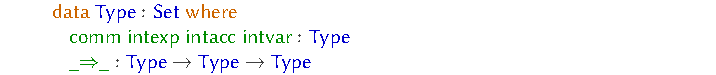
\includegraphics[scale=1.2]{/source/types.pdf}\]

        \subsubsection{Subtypes}
        We use the preorder $A \leq: B$ to denote the subtype relation $A$ is a subtype of $B$, as it has the following properties:
        \begin{itemize}
            \item 
                reflexivity: $A \leq: A$;
            \item 
                transitivity: if $A \leq: B$ and $B \leq: C$, then $A \leq: C$.
        \end{itemize}

        The source language has the following subtype relations:
        \[ \textsf{intvar} \leq: \textsf{intexp} \qquad \textsf{intvar} \leq: \textsf{intacc} \]
        and for function types we have the contravariant subtyping:
        \[ A' \leq: A \land B \leq: B' \Rightarrow A \to B \leq: A' \to B' \]
        
        it is defined in Agda as follows:
        \[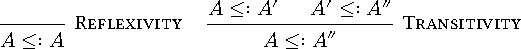
\includegraphics[scale=1.2]{/source/subtype.pdf}\]

        \subsection{Contexts, variables and the lookup judgement}
        We define the context as a finite list of types. When we are looking up a variable, the type of the variable is either on the top of the context or in the tail of the context. The context and the lookup judgement are defined as follows:
        \[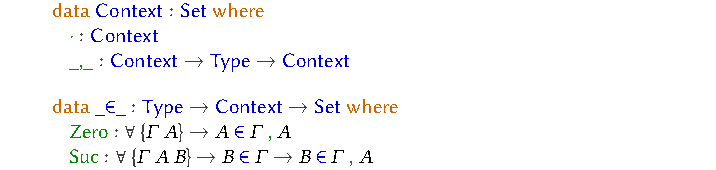
\includegraphics[scale=1.2]{/source/contexts.pdf}\]


        \subsection{Terms and the typing judgement}
        The terms and the typing judgement are described in the following rules:
        \begin{itemize}
            \item For any variable we have 
                \[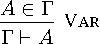
\includegraphics{source_terms_var.pdf}\]
            \item For subtyping we have
                \[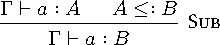
\includegraphics{source_terms_subtype.pdf}\]
            \item For lambda abstraction we have
                \[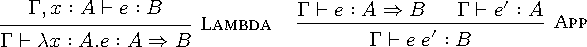
\includegraphics{source_terms_lambda.pdf}\]
            \item For command we have
                \[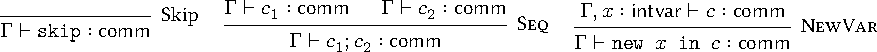
\includegraphics{source_terms_comm.pdf}\]
            \item For integer expression we have
                \[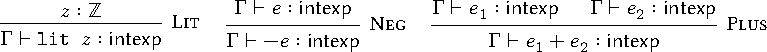
\includegraphics{source_terms_intexp.pdf}\]
        \end{itemize}

        The corresponding Agda implementation is as follows, note that the Agda implementation does not include the name of the terms, but the names are included in the latex implementation for clarity:
        \[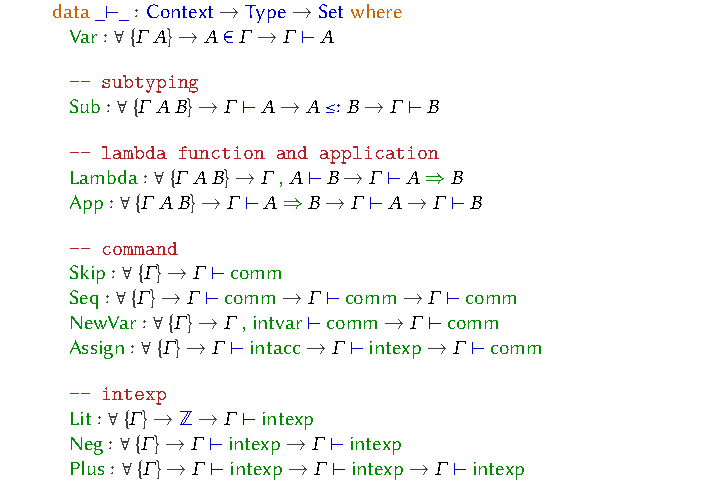
\includegraphics[scale=1.2]{/source/terms.pdf}\]

        Here the definition of the integers is defined in the customised library, which is defined in [section ref].

        \subsection{Operational Semantics}
        The operational semantics of the source language is defined with renaming, substitution and reduction rules. However, since the compiler itself does not require the operational semantics, the implementation is included in the appendix [link to appendix]. Operational semantics can be used to verify the correctness of the compiler in the future, but it is beyond the scope of this dissertation.


    \section{Target Language}
    The target language is an assembly-style intermediate language for a stack machine. It is defined with four stack-descriptor-indexed families of non-terminals: 
    \begin{itemize}
        \item 
            $\bracket{\textsf{L}_{sd}}$: lefthand sides
        \item 
            $\bracket{\textsf{S}_{sd}}$: simple righthand sides
        \item
            $\bracket{\textsf{R}_{sd}}$: righthand sides
        \item
            $\bracket{\textsf{I}_{sd}}$: instruction sequences
    \end{itemize}

    \subsection{Stack descriptor}
    The stack descriptor $sd$ is defined as a pair of natural numbers $\ang{f, d}$, where $f$ is the frame number and $d$ is the displacement. 

    It is defined in Agda as follows:
    \[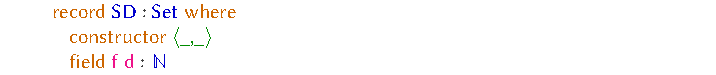
\includegraphics[scale=1.2]{/target/stack_descriptor.pdf}\]
    This requires the definition of natural numbers, which is defined in \secref{subsec: natural_numbers}.

    For a stack descriptor $sd$, we can use \dpink{SD.f} $sd$ to access the frame number and \dpink{SD.d} $sd$ to access the displacement. 

    \subsubsection{Order}
    The stack descriptor is ordered lexicographically with $\leq_s$ as follows:
    \[\ang{f, d} \leq_s \ang{f', d'} \Leftrightarrow f < f' \lor (f = f' \land d \leq d')\]

    It is defined in Agda as follows:
    \[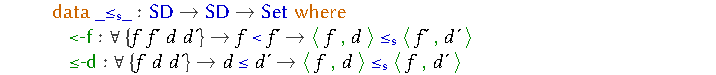
\includegraphics[scale=1.2]{/target/stack_descriptor_order.pdf}\]
    This requires the definition of the order of natural numbers, which is defined in \secref{subsec: order}.

    \subsubsection{Addition and subtraction of stack descriptors}
    We define addition and subtraction of stack descriptors as follows:
    \[\ang{f, d} \pm_s n = \ang{f, d \pm n} \text{ for } n \in \mathbb{N}\]
    Addition of stack displacement is defined in Agda as follows:
    \[
\includegraphics[scale=1.2]{/target/stack_descriptor_add.pdf}\]
    For subtraction, we need to make sure that the subtraction is valid, i.e. the subtracted displacement is less than or equal to the displacement of the current stack descriptor. Here we need a rigorous definition of the subtraction of natural numbers, which is defined in \secref{subsec: subtraction}

    \subsubsection{Properties of order and addition}
    We can use reflexivity and transitivity of the order $<$ and $\leq$ to prove that the order of stack descriptors $\leq_s$ is a preorder. The proof is as follows:
    \begin{itemize}
        \item 
            Reflexivity: $sd \leq_s sd$ is trivially true since $f = f$ and $d \leq d$.
        \item
            Transitivity: if $\ang{f, d} \leq_s \ang{f', d'}$ and $\ang{f', d'} \leq_s \ang{f'', d''}$, we do the following case split:
            \begin{itemize}
                \item 
                    if $f < f'$, $f' = f''$ and $d \leq d'$, then $f < f''$; 
                \item 
                    if $f < f'$ and $f' < f''$, then $f < f''$ by transitivity of $<$;
                \item
                    if $f = f'$, $d \leq d'$ and $f' < f''$, then $f < f''$;
                \item
                    if $f = f'$, $d \leq d'$, $f' = f''$ and $d' \leq d''$, then $f = f''$ and $d \leq d''$ by transitivity of $\leq$. \footnote{Note that the properties of $=$ is not required in as in the Agda definition of $\leq_s$, we directly define $f'$ to be $f$ instead of defining a equivalence relation, thus equivalence can be checked directly via type checking.}
            \end{itemize}
    \end{itemize}
    The proof is defined in Agda as follows:
    \[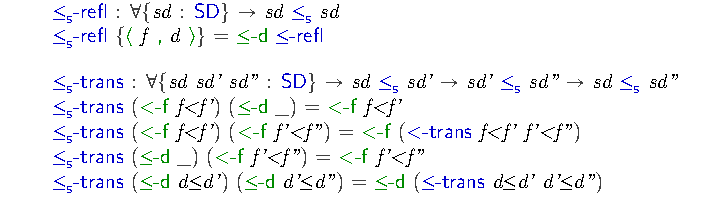
\includegraphics[scale=1.2]{/target/stack_descriptor_order_proof.pdf}\]

    When a natural number is added to a stack descriptor, it is guaranteed that the new stack descriptor is not less than the old stack descriptor. This can be proved directly using the same properties of integer addition. The proof is defined in Agda as follows:
    \[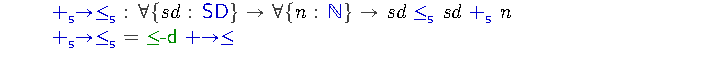
\includegraphics[scale=1.2]{/target/stack_descriptor_add_proof.pdf}\]

    Proof above requires the proof of the properties of natural numbers, which is defined in [section ref].
    

    \subsection{Grammar}
    The grammar of the target language is defined as follows, given the current stack descriptor $sd = \ang{f, d}$, and new stack descriptor $sd' = \ang{f', d'}$:
    \[\begin{aligned}
        \bracket{\textsf{L}_{sd}} ::={}& sd^v \quad \text{when } sd^v \leq_s sd \\
                        &\mid \texttt{sbrs}  \\
        \bracket{\textsf{S}_{sd}} ::={}& \bracket{\textsf{L}_{sd}} \\
                        &\mid \texttt{lit} \bracket{\text{integer}} \\
        \bracket{\textsf{R}_{sd}} ::={}& \bracket{\textsf{S}_{sd}} \\
                        &\mid \bracket{ \text{unary operator} } \bracket{ \textsf{S}_{sd}}\\
                        &\mid \bracket{\textsf{S}_{sd}} \bracket{\textsf{binary operator}} \bracket{ \textsf{S}_{sd} } \\
        \bracket{\textsf{I}_{sd}} ::={}& \texttt{stop} \\
                        &\left.
                        \begin{aligned}
                        &\mid \bracket{\textsf{L}_{sd+\delta}} \gets \bracket{\textsf{R}_{sd}}[\delta] \text{ ; } \bracket{\textsf{I}_{sd+\delta}} \\
                        &\mid \texttt{if } \bracket{\textsf{S}_{sd}} \bracket{\text{relational operator}} \bracket{\textsf{S}_{sd}}[\delta] \\
                        & \hphantom{\mid {}} \texttt{ then } \bracket{\textsf{I}_{sd+\delta}} \texttt{ else } \bracket{\textsf{I}_{sd+\delta}} \\
                        &\mid \texttt{adjustdisp} [\delta] \text{ ; } \bracket{\textsf{I}_{sd+\delta}} \\
                        \end{aligned}
                        \quad \right\} \text{if } d + \delta \geq 0  \\
                        &{}\mid \texttt{popto } sd' \text{ ; } \bracket{\textsf{I}_{sd'}} \quad \text{when } sd' \leq_s sd \\
    \end{aligned}\]

    \subsubsection{Operators}
    The operators are defined as follows:
    \[\begin{aligned}
        \textsf{unary operator} &\in \{\texttt{UNeg}\} \\
        \textsf{binary operator} &\in \{\texttt{BPlus}, \texttt{BMinus}, \texttt{BTimes}\} \\
        \textsf{relational operator} &\in \{\texttt{RLeq}, \texttt{RLt}\}
    \end{aligned}\]

    The operators are defined in Agda as follows:
    \[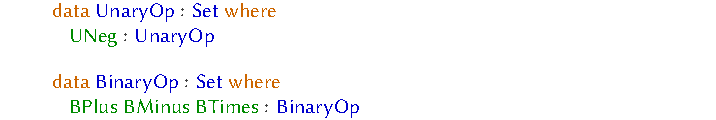
\includegraphics[scale=1.2]{/target/operators.pdf}\]

    \subsubsection{Lefthand sides, simple righthand sides and righthand sides}
    The lefthand sides, simple righthand sides and righthand sides are straightforward, and they are defined as follows in Agda:
    \[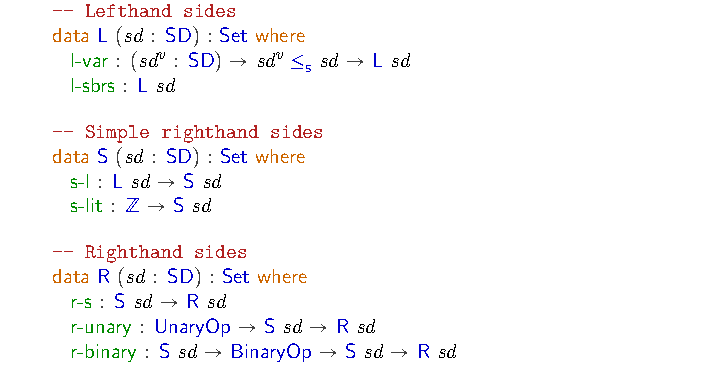
\includegraphics[scale=1.2]{/target/leftrighthand_sides.pdf}\]

    \subsubsection{Instruction sequences}
    In the instruction sequences, $\delta$ as a displacement can be either positive or negative. To make a rigorous definition, we define $\delta$ as a natural number, and treat the positive and negative displacements as two different instructions, using addition and subtraction of stack descriptors respectively. Since the definition of negative displacement involves the rigorous definition of subtraction, we will discuss the subtraction of natural numbers and correpsonding implementation in \secref{subsec: subtraction}. The definition (except for the negative displacement) in Agda is as follows:
    \[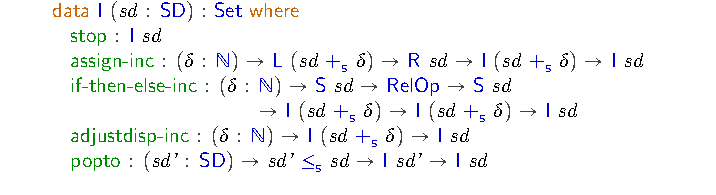
\includegraphics[scale=1.2]{/target/instruction_inc.pdf}\]


    \section{Customised Library}
    The customised library is a collection of types and functions centered around natural numbers, their operations and properties. 

    \subsection{Natural numbers, integers and addition} \label{subsec: natural_numbers}
    The definition of natural numbers, integers and addition is standard, and it is defined as follows:
    \[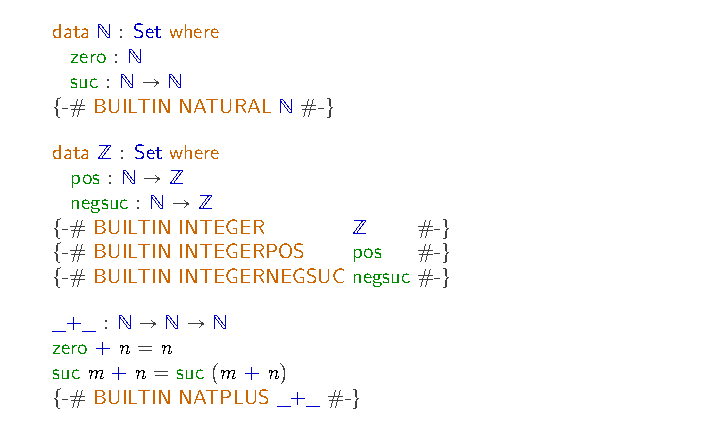
\includegraphics[scale=1.2]{/lib/natural.pdf}\]
    The use of \og{\textsf{BUILTIN}} is specifed in \secref{subsubsec: builtin_pragma}.

    \subsection{Equality, congruence and substitution}
    The definition of equality, congruence and substitution is similar to the one in \secref{subsec: equality}.\footnote{The definition of equality and related properties in the custom library differ slightly by using an indexed $\mb{\mathsf{Set}}$, which provides a more general formulation. See Appendex [corresponding link].}

    \subsection{Order of natural numbers} \label{subsec: order}
    The order of natural numbers we defined include $\leq$ and $<$, which are defined standardly as follows:
    \[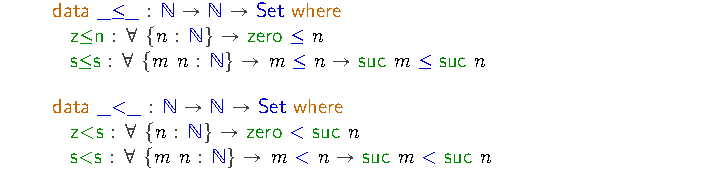
\includegraphics[scale=1.2]{/lib/order.pdf}\]

    \subsection{Properties of order and addition}
    \subsubsection{Transitivity and reflexivity}
    The transitivity and reflexivity of the order $<$ and $\leq$ are defined as follows:
    \[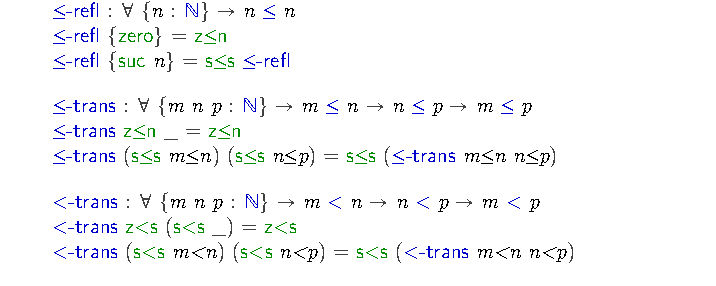
\includegraphics[scale=1.2]{/lib/order_proof.pdf}\]

    \subsubsection{Implication of order}
    We know that $\forall m, n \in \bN$, if $m < n$, then we have $m + 1 \leq n$ and $m \leq n$. This is defined in Agda as follows:
    \[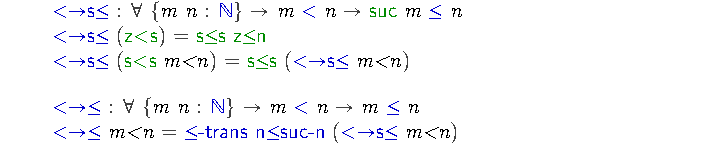
\includegraphics[scale=1.2]{/lib/order_implication.pdf}\]

    \subsubsection{Totality of order}
    It is useful to case split the order of natural numbers, i.e. for any $m, n \in \bN$, we have $m \leq n$ or $n \leq m$. This is defined in Agda by defining either case as an instance of the \mb{\textsf{Total}} type, and then showing that for any $m, n \in \bN$, we can construct a \mb{\textsf{Total}} type by case-split and \og{\textsf{with}}-construct. The proof is as follows:
    \[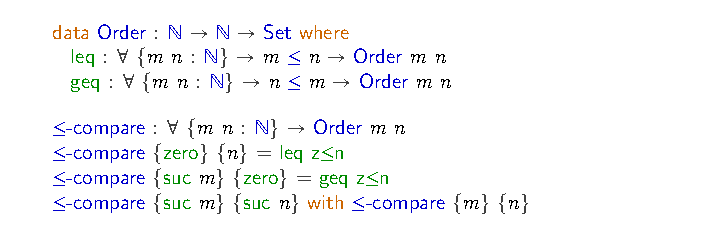
\includegraphics[scale=1.2]{/lib/order_totality.pdf}\]


    \subsubsection{Other properties}
    We can show that when a number $n$ is added to a natural number $m$, the result is greater than or equal to $m$. This is defined in Agda as follows:
    \[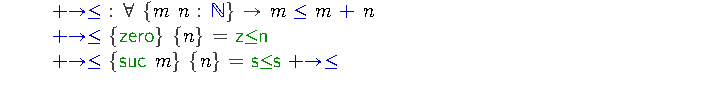
\includegraphics[scale=1.2]{/lib/order_add.pdf}\]


    \subsection{Subtraction} \label{subsec: subtraction}
    In the standard library~\cite{agda_std}, the subtraction of natural numbers is defined as follows:\footnote{The definition in the standard library directly uses symbol $\mathsf{-}$, but here for clarity we use $\mathsf{\dotdiv}$ instead.}
    \[\includegraphics[scale=1.2]{minus.pdf}\]
    Mathematically we have $ n \dotdiv m = \max(0, n - m)$. This definition is valid and ensures that the result is a natural number. However, there are two problems with this definition for our implementation:
    \begin{itemize}
        \item 
            The definition of subtraction is not rigorous. Input $n$ should be guaranteed not to be less than $m$, and at any point in the program if there is a subtraction where $n < m$, the program should fail to type check instead of making $0$ type check with it.
        \item
            We lose many numerical properties of natural numbers. For example, $n \dotdiv m + m = n$ or $n \dotdiv (n \dotdiv m) = m$ are not guaranteed to hold if we allow $n < m$. Those properties are very useful for the implementation of the compiler.
    \end{itemize}
    We need a more rigorous definition of subtraction that ensures the result is a natural number and preserves the numerical properties. The key is to have a proof that the first argument is greater than or equal to the second argument. There are two approaches to achieve this:

    \subsubsection{Explicit proof-passing approach}
    A straightforward approach is directly include a third argument in the subtraction function, which is a proof that the first argument is greater than or equal to the second argument. The definition in Agda is as follows:
    \[\includegraphics[scale=1.2]{/lib/proof/minus.pdf}\]

    The corresponding implementation for subtraction of stack descriptors carries along the proof as follows:
    \[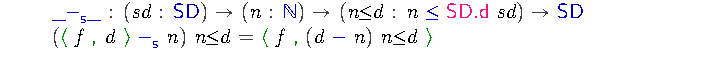
\includegraphics[scale=1.2]{/target/proof/stack_descriptor_minus.pdf}\]

    In the implementation of instruction sequences, we need to carry along the proof as well. The implementation in Agda is as follows:
    \[\includegraphics[scale=1.2]{/target/proof/instruction_dec.pdf}\]

    \subsubsection{\textsf{Fin}-based approach}
    Instead of include the proof directly, we can define the type of the subtrahend as a type that depends on the minuend, where the type encodes the proof. There is a standard library in Agda on finite sets, where a type $\mb{\mathsf{Fin}}$ is defined as a type that depends on a natural number $n$, where $\mb{\mathsf{Fin}}\ n$ can be seen as the set of natural numbers less than $n$. The definition is as follows:
    \[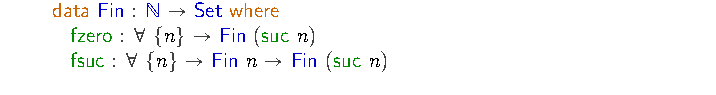
\includegraphics[scale=1.2]{/lib/fin/fin.pdf}\]

    An intuitive explanation of the definition of $\mb{\mathsf{Fin}}$ is as follows:
    \begin{itemize}
        \item Base case: when $n = 0$, there is no element less than $0$, so we do not have any constructor that gives us an element of type $\mb{\mathsf{Fin}}\ 0$. 
        \item Inductive case: 
        \begin{figure}[H]
            \centering
            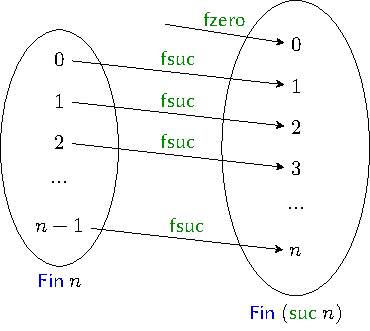
\includegraphics[width=0.35\textwidth]{fin_inductive.pdf}
            \caption{Inductive case of $\mb{\mathsf{Fin}}$}
            \label{fig: fin_inductive}
        \end{figure}
    \end{itemize}

    For subtraction, we only need to change the type of the subtrahend to $\mb{\mathsf{Fin}}\ (\gn{\mathsf{suc}}\ n)$ compared to the implementation of addition. The definition in Agda is as follows:
    \[\includegraphics[scale=1.2]{/lib/fin/minus.pdf}\]

    The corresponding implementation for subtraction of stack descriptors and instruction sequences only requires a change of the type of the subtrahend as follows:
    \[\includegraphics[scale=1.2]{/target/fin/instruction_dec.pdf}\]

    \subsubsection{Comparison of the two approaches}
    The straightforward approach explicitly carries proofs in the type system, which is more transparent but verbose. The fin approach intially appears to be more elegant, as it encapsulates bounds check within a refined type. However, this elegance is superficial: constructing a term of type $\mb{\mathsf{Fin}}\ n$ still requires the same underlying proof of boundedness, shifting complexity to auxiliary conversions. 
    
    To prove a property with the fin approach, we need the following auxiliary function:
    \[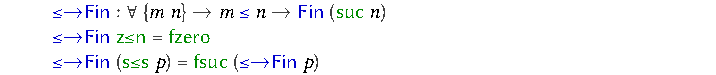
\includegraphics[scale=1.2]{/lib/fin/toFin.pdf}\]

    Here is a comparison of the two approaches representing the property $\mathsf{suc}\ (n - m) \equiv \mathsf{suc}\ n - m$:
    \begin{figure}[H]
        \centering
        \includegraphics[scale=1.2]{/lib/proof/minus-suc.pdf}
        \includegraphics[scale=1.2]{/lib/fin/minus-suc.pdf}
        \caption{Comparison of explicit vs. \textsf{Fin}-based approaches}
        \label{fig: fin_comparison}
    \end{figure}
    It is clear that the explicit proof-passing approach is more straightforward and easier to understand. The fin-based approach requires additional auxiliary functions and conversions, which makes the code more complex and harder to read.

    Although the project completed both approaches, the following implementation of the compiler uses the explicit proof-passing approach due to its simplicity and clarity.

    \subsection{More properties of natural numbers}


    

    \section{Compiler}




\chapter{Evaluation}
    \minitoc
    Chapter~\chapref{chap: implementation} describes the implementation of the source language, the target language and the compiler in Agda. This chapter evaluates the implementation with a demonstrative example in Agda, and discusses the success criteria of the project.
    \section{A demonstrative example in Agda}

    \section{Success criteria}

\chapter{Conclusion}
    \minitoc
    \section{Results}

    \section{Overview}

    \section{Lessons learned}

    % \section{Future work}

\printbibliography

\appendix

\cleardoublepage
\let\cleardoublepage\clearpage
\pagestyle{empty}
\pagenumbering{gobble}
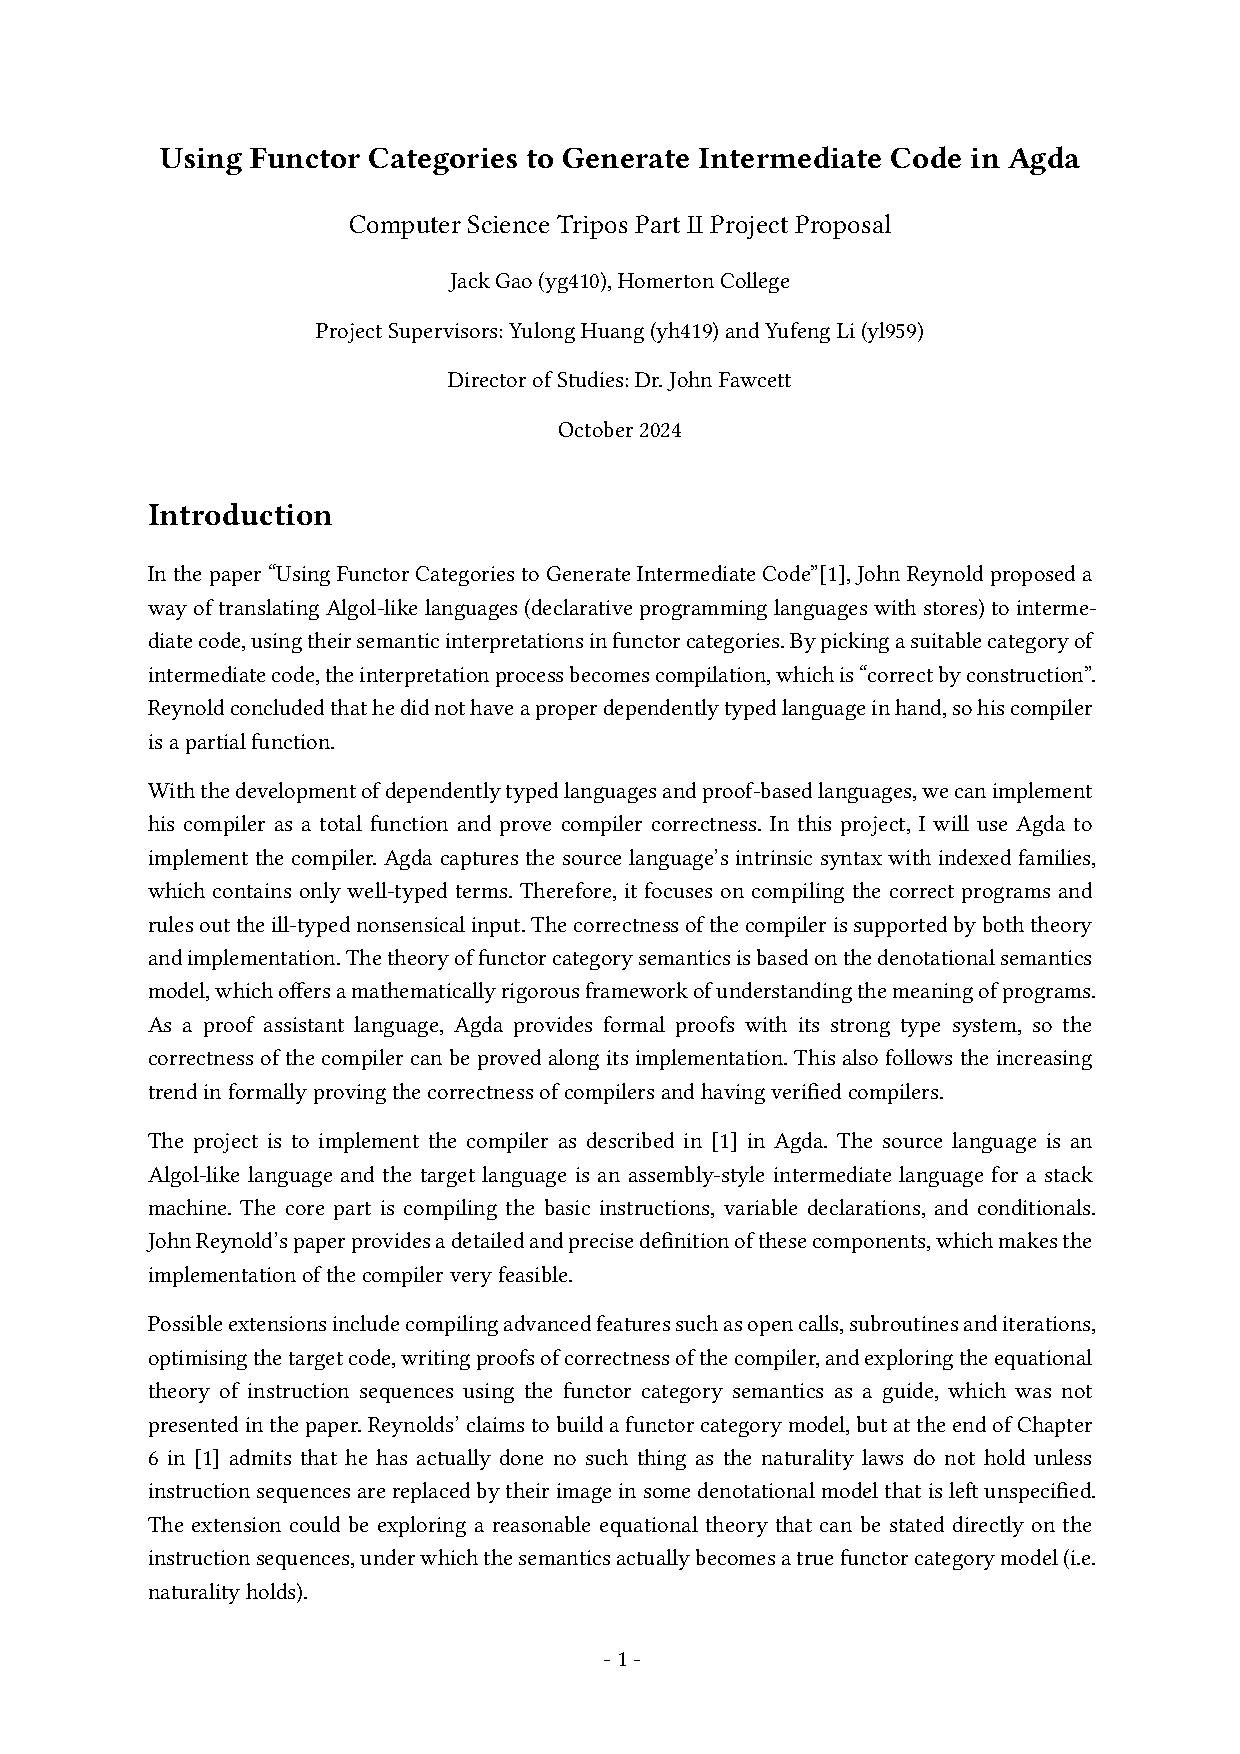
\includepdf[pages=-, fitpaper=true, pagecommand={}]{final_proposal.pdf}
\AtBeginShipoutNext{\AtBeginShipoutDiscard}
\end{document}